\section{Result and Evaluation} \label{sec:eval}
This section discuss the result of the simulation with our implemented lattice Boltzmann method on SpiNNaker. Firstly, the evaluation setup (\ref{sec:es}) including the serial version and SpiNNaker version would be discussed. Then we will discuss the correctness and the accuracy of simulation in different scale at \ref{sec:caae}. Then we will compare the performance in term of speed with the serial implementation in CPU at \ref{sec:perfe}.
\subsection{Evaluation Setup} \label{sec:es}
In this project, we used a serial implementation of the test problem in C as the baseline. The serial version run on EPCC's computing facility Cirrus (Intel Xeon E5-2695 (Broadwell)), with no compiler optimization.\\

On the SpiNNaker side, we run our simulation on the SpiNNaker cluster in the University of Manchester, which contains 1,036,800 cores, via the SpiNNaker Jupyter Notebook interface. \\

For evaluation, we use three different scale of simulation; see \ref{table:setting}. We will firstly plot the contour graph of the result of those three simulation. Those simulation indicate the same problem but in different resolution. Then we will use the normalized distances L-1 norm, L-2 norm and L-infinite norm  of (1) SpiNNaker version vs. Serial float version; (2) SpiNNaker version vs. Serial double version; (3) Serial float version vs. Serial double version to discuss the correctness and the accuracy of our SpiNNaker implementation.\\

\begin{table}[tb]
\centering
\begin{tabular}{|c|c|c|c|}
\hline
Scale          & 64$\times$64 & 128$\times$128 & 256$\times$256 \\ \hline
total cores    & 4086         & 16384          & 65536          \\ \hline
total timestep  & 5120         & 10240          & 20480          \\ \hline
$\nu$           & 0.000064     & 0.000128       & 0.000256       \\ \hline
$\tau$           & 0.500192     & 0.500384       & 0.500735       \\ \hline
\end{tabular}
\caption{The physical parameters setting in three different scales.}
\label{table:setting}
\end{table}


For performance, in this project, we focus on speed. To more visually compare the magnitude of the relationship between them, after confirmed the correctness, we do not take physical settings into consideration. In other words, all the experiments of those three scale would run for 12000 time steps. We will compare the total simulation time and the simulation time per time step of the SpiNNaker implementation and serial implementation in the three scales. \\

It should be noted that, in SpiNNaker, we do not take the time spend on loading SpiNNaker hardware configuration into account for the above comparison. We will discuss it as well as other limitation of this implementation in more detail at \ref{sec:ana}.\\

Finally, an analysis would be given to the challenge we faced during this project, including some technical difficulties and some general difficulties caused by the COVID-19.

To make the results more plausible, we took the tie value for three executions for every result.\\
\subsection{Correctness and Accuracy Evaluation} \label{sec:caae}
Firstly, we can get an general judgement on the correctness from the vorticity contour. In Fig.~\ref{fig:contour}, Fig.~\ref{fig:a},Fig.~\ref{fig:c} and Fig.~\ref{fig:e} is produced from the serial C implementation in double floating precise. According to \cite{minion1997performance}, with its configuration, there would be a turbulence in the periodic system. It is clear that there are turbulence in all three scale. Turbulence is recognized as a complex system and if there is any small error during the calculation, eventually, the result would be markedly different. In this case, we got a similar turbulence as \cite{minion1997performance}; and now We are confident enough that our serial implementation is correct.\\

On the left hand side of Fig.~\ref{fig:contour}, we have the contour result from the SpiNNaker implementation. It is clear that the result from the SpiNNaker implementation has similar contours as the serial C implementation. And it is noticeable that there are some noises in low-resolution contour i.e.$64\times64$ simulation and the noises decreases when the resolution increase, which fits what we were expecting before the simulation. We can now say that our implementation is correct. However, CFD need accuracy and if we want to know how accurate our simulation is, we need to analysis the result numerically.\\

\begin{figure}[htbp]  
\begin{subfigure}{0.43\textwidth}
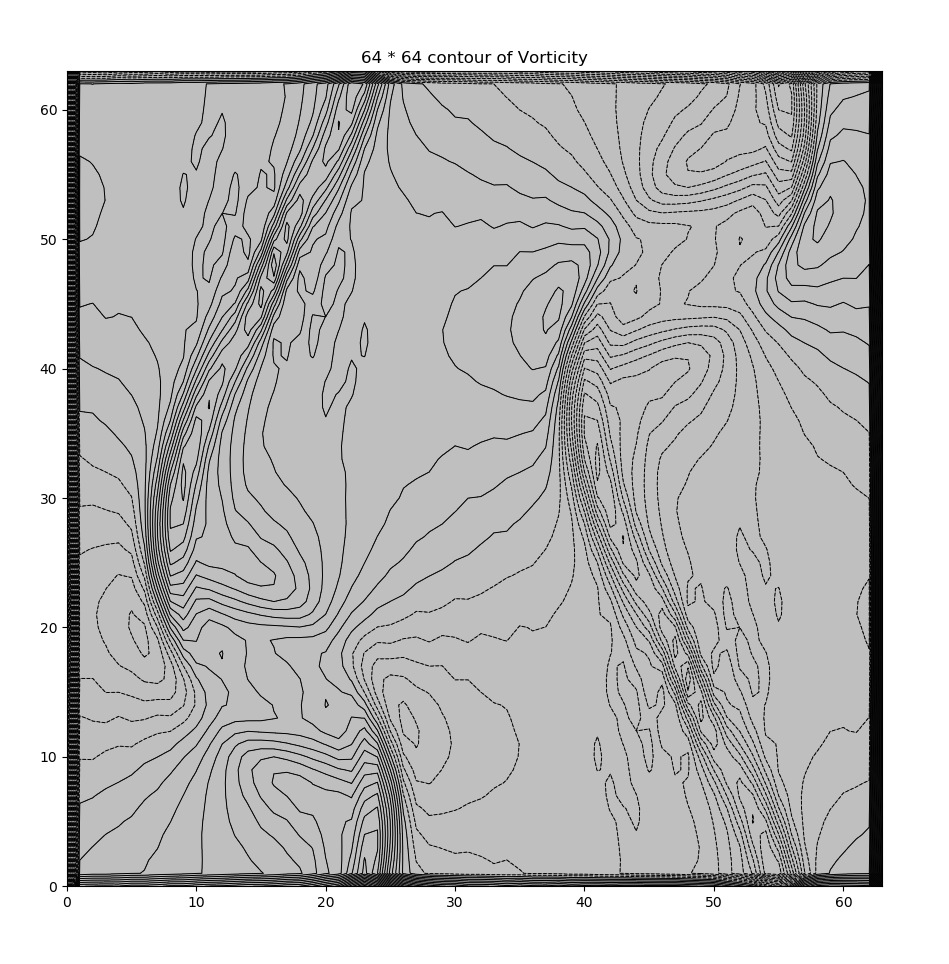
\includegraphics[width=\linewidth]{figures/double_c_64.png}
\caption{Contour of 64$\times$64 from serial C implementation} \label{fig:a}
\end{subfigure}\hspace*{\fill}
\begin{subfigure}{0.57\textwidth}
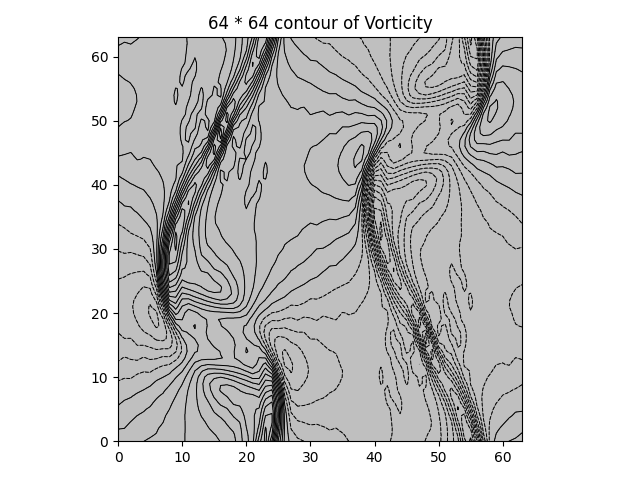
\includegraphics[width=\linewidth]{figures/spinnaker_64.png}
\caption{Contour of 64$\times$64 from SpiNNaker implementation} \label{fig:b}
\end{subfigure}

\medskip
\begin{subfigure}{0.43\textwidth}
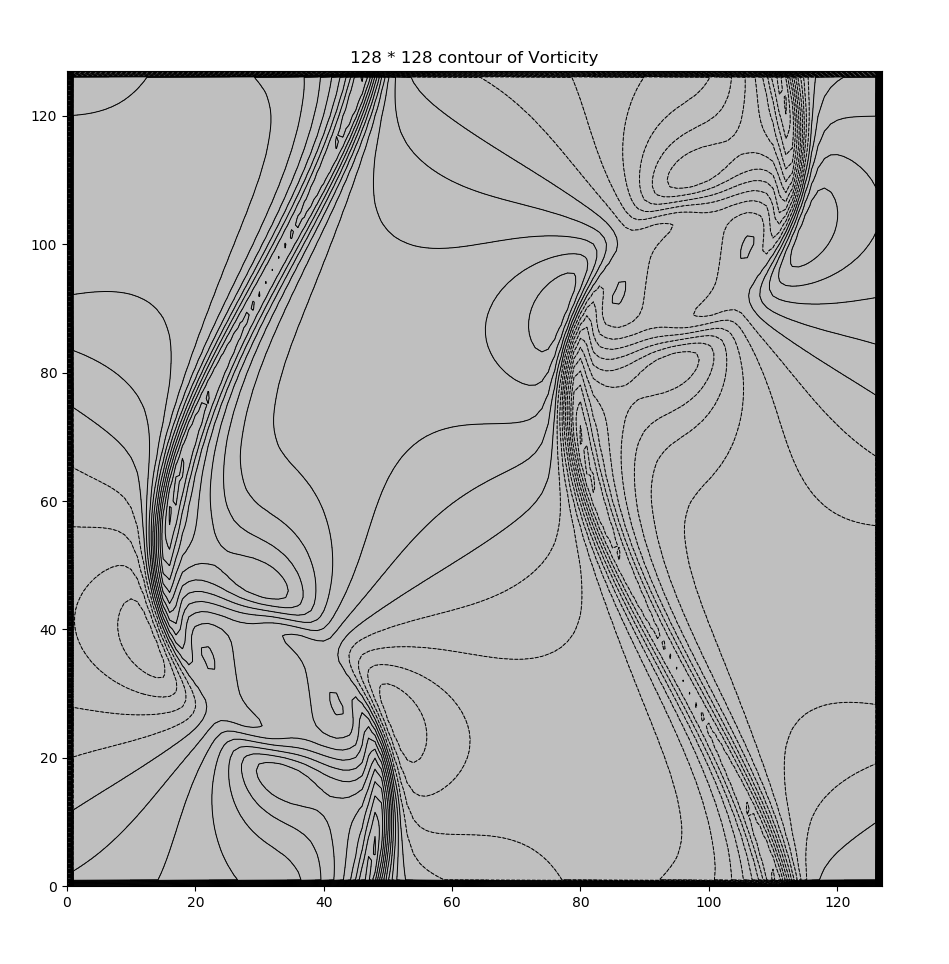
\includegraphics[width=\linewidth]{figures/double_c_128.png}
\caption{Contour of 128$\times$128 from serial C implementation} \label{fig:c}
\end{subfigure}\hspace*{\fill}
\begin{subfigure}{0.57\textwidth}
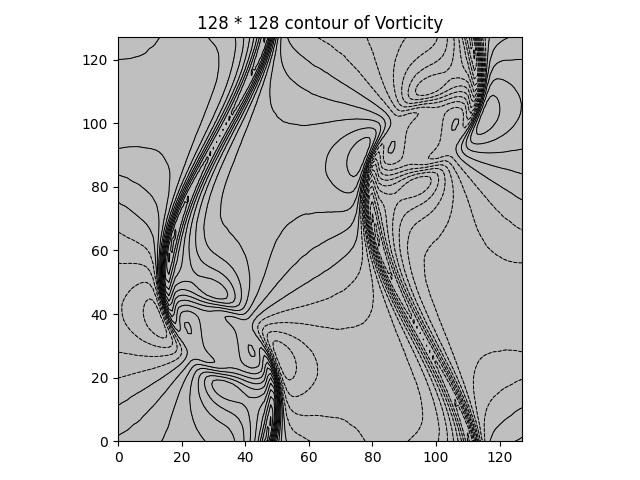
\includegraphics[width=\linewidth]{figures/spinnaker_128.png}
\caption{Contour of 128$\times$128 from SpiNNaker implementation} \label{fig:d}
\end{subfigure}

\medskip
\begin{subfigure}{0.43\textwidth}
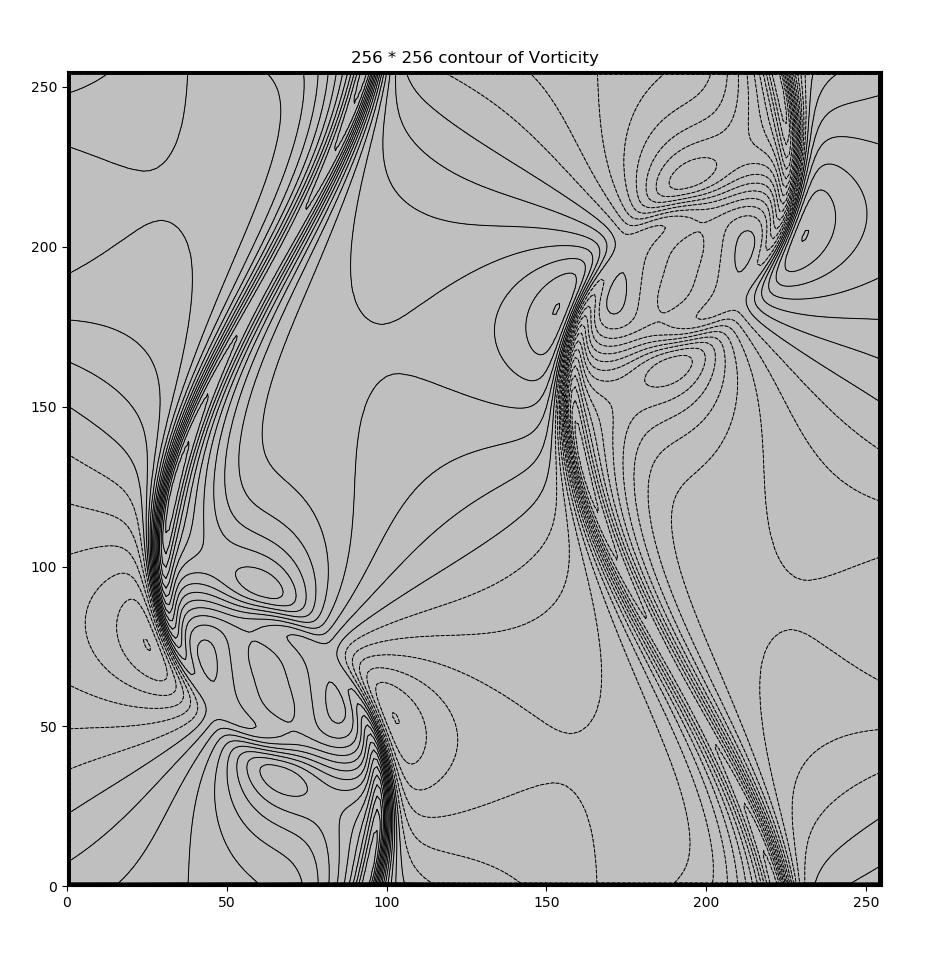
\includegraphics[width=\linewidth]{figures/double_c_256.png}
\caption{Contour of 256$\times$256 from serial C implementation} \label{fig:e}
\end{subfigure}\hspace*{\fill}
\begin{subfigure}{0.57\textwidth}
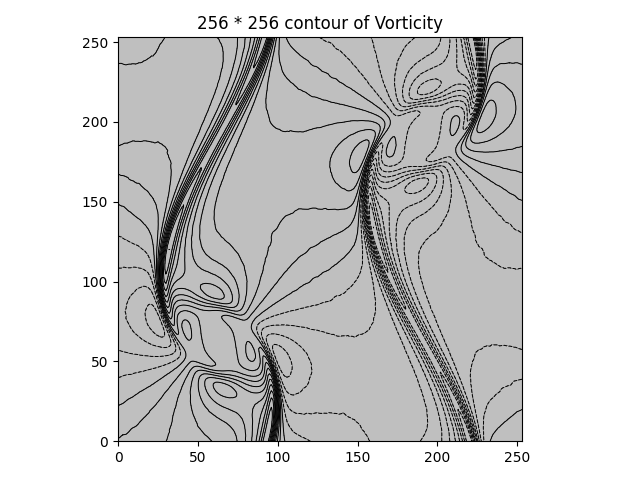
\includegraphics[width=\linewidth]{figures/spinnaker_256.png}
\caption{Contour of 256$\times$256 from SpiNNaker implementation} \label{fig:f}
\end{subfigure}
\caption{Contour graphs of the simulations in three different resolution. \ref{fig:a},\ref{fig:c},\ref{fig:e} are the contour graph with scale of $32\times32$, $64\times64$ and $128\times128$ from serial C implementation in double floating precise.\ref{fig:b},\ref{fig:d},\ref{fig:f} are the contour graph with scale of $32\times32$, $64\times64$ and $128\times128$ from SpiNNaker implementation.} 
\label{fig:contour}
\end{figure}

In Table.~\ref{table:norm}, we show how we quantifying the variation between different results. We can regard the double precis serial C version as a baseline and compare it with the floating-point implementation in serial C. From the table, it is clear that in terms of $L-$ norm, $L-2$ norm and $L_{infi}$, SpiNNaker implementation maintained at the same level as C. More specifically, we introduced another criteria, the L-2 norm per grid, to quantify effect of error on each grid; and the L-2 per grid of SpiNNaker implementation also stay at the same level of floating-point C implementation. Therefore, we can confirm that, in terms of accuracy, SpiNNaker's LBM implementation is already at the level of existing CPUs.\\

\begin{table}[tb]
\begin{tabular}{|c|c|c|c|c|}
\hline
Scale                & Norm        & float vs. double& float vs. SpiNNaker& double vs. SpiNNaker\\ \hline
\multirow{4}{*}{64}  & L-1          & 3.14e-03             & 4.47e-03              & 3.63e-03               \\ \cline{2-5} 
                     & L-2          & 6.34e-05           & 9.13e-05          & 7.51e-05           \\ \cline{2-5} 
                     & $L_{infi}$  & 4.20e-06           & 6.61e-06          & 5.88e-06           \\ \cline{2-5} 
                     & L-2 per Grid & 1.55e-08          & 2.23e-08           & 1.83e-08            \\ \hline
\multirow{4}{*}{128} & L-1          & 1.26e-02             & 1.36e-02              & 1.52e-02               \\ \cline{2-5} 
                     & L-2          & 1.26e-04             & 4.48e-02              & 1.52e-04               \\ \cline{2-5} 
                     & $L_{infi}$  & 4.50e-06          & 4.42e-06          & 5.74e-06           \\ \cline{2-5} 
                     & L-2 per Grid & 7.69e-08          & 2.73e-06           & 9.28e-09            \\ \hline
\multirow{4}{*}{256} & L-1          & 4.74e-02             & 5.61e-02              & 3.22e-02               \\ \cline{2-5} 
                     & L-2          & 2.39e-04             & 2.78e-04              & 1.42e-04               \\ \cline{2-5} 
                     & $L_{infi}$  & 4.30e-06         & 4.80e-06           & 9.00e-06           \\ \cline{2-5} 
                     & L-2 per Grid & 1.43e-08           & 1.80e-08            & 9.09e-09              \\ \hline
\end{tabular}
\caption{A chart of three different matrix norm between each two of floating-point C, double precis floating-point C and SpiNNaker. Here we use L-1 norm, L-2 norm and L-infinite norm to quantify the extent of variation in results. Besides, we introduce another criteria L-2 norm per grid to quantify the variation of each lattice.}
\label{table:norm}
\end{table}

\subsection{Performance Evaluation} \label{sec:perfe}
After quantifying the correctness and the accuracy, we now have a reasonably correct implementation. Then To make it easier to measure its performance, we execute the simulation with different scale in the same time step i.e. 12000 steps.\\

\begin{figure}[tb]
   \centering
       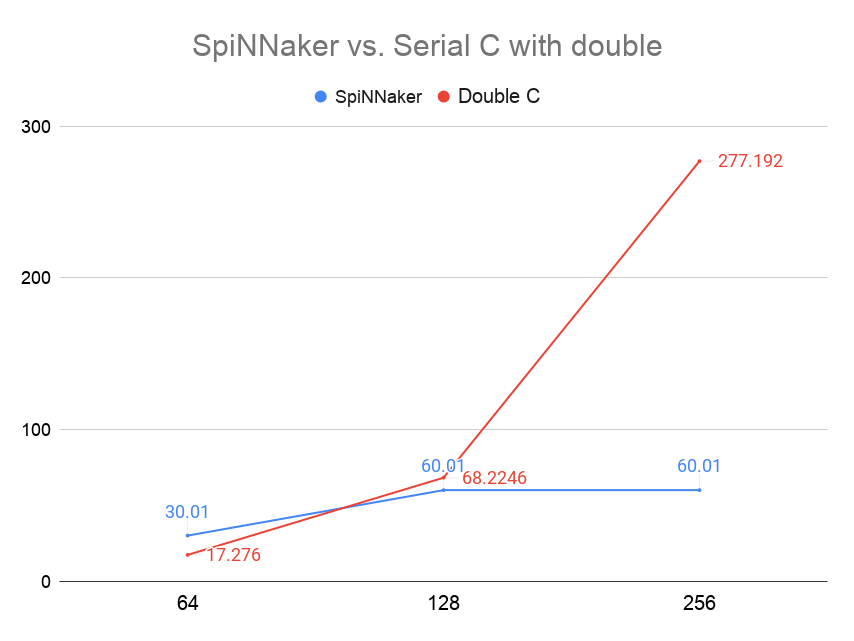
\includegraphics[width=0.8\textwidth]{figures/SpiNNaker vs. Serial C with double.png}
       \caption{Execution time of 12000 time steps in scale of $64\times64$, $128\times128$ and $256\times256$ with SpiNNaker implementation and serial implementation. It should note that the SpiNNaker's performance may not be optimal in this case.}
       \label{fig:performance}
\end{figure}

As Fig.~\ref{fig:performance} shows, as the size of the simulation increases, the execution time of the serial program increases rapidly. When the simulation size is small, the serial program executes more efficiently than SpiNNaker; however, as the task size increases, the SpiNNaker naturally implementation utilizes more cores and gets better performance accordingly. For $128X\times128=16384$ simulation, the speed-up is $60.01/68.224\approx1$, while for $256\times256=65536$ simulation, the SpiNNaker gain $277.192 / 60.01 = 4.61$ speed-up. As the simulation scale increase by $65536 / 16384 = 4$ times, the speed-up increase $4.61 / 1 = 4.61$ times. Therefore, as the With this implementation and hardware, we achieve a relatively good weak-scaling performance.\\

It is noticeable that in SpiNNaker $128\times128$ simulation and $256\times256$ simulation need the same amount of time. This is because: (1) in this project, we only allocate 1 lattice per core. And as the scale of simulation increase, the SpiNNaker implementation will correspondingly increased use of cores; (2) in this project, we have not yet get the optimal performance of SpiNNaker, especially for $128\times128$ simulation. To get a better performance, we are supposed to adjust the SpiNNaker configuration, e.g. timer offset, time scale factor, delay between multicast, really carefully, which need time that beyond the scope of this project.


\subsection{Limitation Evaluation} \label{sec:ana}
The first limitation is from the device itself. In the previous performance analysis, we only take the time spend on \textbf{simulation}, which means we do not take the non-simulation time ,e.g. booting the machine, loading data specification to the device, loading data back to host etc., into account. In fact, with the increasing scale of the simulation, the time spend on the non-simulation tasks become larger; see Fig.~\ref{fig:loading}.\\

\begin{figure}[tb]
   \centering
       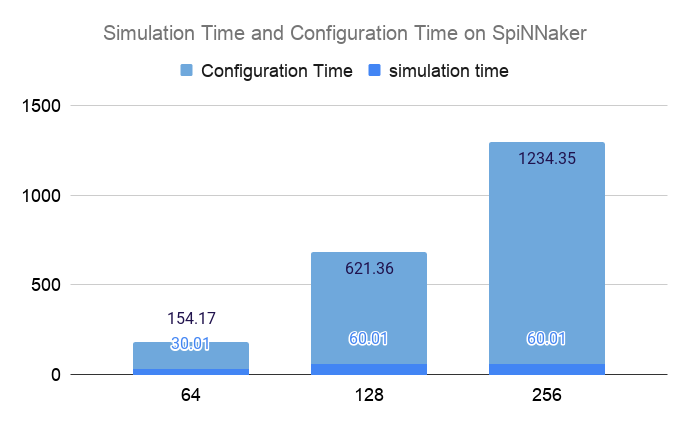
\includegraphics[width=0.8\textwidth]{figures/Simulation Time and Configuration Time on SpiNNaker.png}
       \caption{Simulation time and the configuration time for three different scale simulation. From the chart, it is clear that as the increasing of the simulation scale, there are more time spending on setting up the device and get the simulation result back to host.}
       \label{fig:loading}
\end{figure}

At the moment, it's not possible to solve the problem completely, because as the increasing of simulation scale, there will be more data need to transfer before and after the simulation. However, a group of researchers and engineers are working on tools that enable the SpiNNaker to load data in parallel, which would accelerates data transfer greatly.\\

Another limitation is that, in this project, we only allocate 1 lattice per SpiNNaker core. Although, we can get parallelism from this configuration, the number of available cores significantly limits the upper limit of simulation scale. In this implementation with available SpiNNaker hardware (about 1,000,000), the maximum scale of simulation is around  $1000 \times 1000$, which is not yet sufficient for real-world engineering problems.\\

Finally, we are using the time ticker of SpiNNaker as a trigger of time step. Indeed, it is convenient for a basic implementation. However, the developers need to adjust the timer offset, timing information and maximum of delay between sending the multicast packets really carefully to get a good performance. Especially for larger simulation, e.g. 256$\times$256 simulation in this project, since we are not running simulation on the exactly same cores each time and the physical communication time is not the same from cores to cores, it was time-consuming to find a proper setting.\\

\subsection{Challenge Evaluation}
The very first challenge we faced is SpiNNaker itself. SpiNNaker is a novel architecture with a totally different programming model even for parallel programmers. Getting familiar with the ideas behind SpiNNaker is difficult and one of the difficulties in programming on SpiNNaker is the idea of event-driven asynchronized multicast communication in SpiNNaker. We have predicted it would be difficult in the project preparation but the actual difficulty is beyond our imagine.\\

The second challenge comes from the lock-down caused by the COVID-19. Since SpiNNaker is at the forefront of academia, there is not much discussion about SpiNNaker on the web. Trying to get resources on SpiNNaker relies heavily on talking to Dr Alan Stokes, one of my mentors. However, lock-down has made Alan, who was originally accessible 3 days a week, available on a weekly basis. This makes acquiring prior knowledge about SpiNNaker so hard that I need to turn to the SpiNNaker user group frequently, even though the people in the SpiNNaker user group are great, and this delays the project. \\

The last and most significant challenge across this project comes from the physical board. As we discussed before this report, this project should have proposed an early prototype and then switch to the SpiNNaker cluster for larger simulation. However, the physical board came across some connection problems and for the development efficiency, we directly switch to the Jupyter interface. If there is no lock-down, the repair would be available and the development should be more efficient as it is more straightforward to debug locally and we do not need to compete with the other users and researchers for SpiNNaker cluster usage. The spared time can be used as adjusting the parameters for a better performance or development the multi-lattice-single-core implementation.





